% Hlavicka pro protokoly z fyzikalniho praktika.
% Verze pro: LaTeX
% Verze hlavicky: 22. 2. 2007
% Autor: Ustav fyziky kondenzovanych latek
% Ke stazeni: www.physics.muni.cz/ufkl/Vyuka/
% Licence: volne k pouziti, nejlepe k vcasnemu odevzdani protokolu z Vaseho mereni.


\documentclass[czech,11pt,a4paper]{article}
\usepackage[T1]{fontenc}
\usepackage{graphicx}
\usepackage{mathtools}
\usepackage{amssymb}
\usepackage{amsthm}
\usepackage{thmtools}
\usepackage{xcolor}
\usepackage{nameref}
\usepackage{babel}
\usepackage{hyperref}
\usepackage{multicol}

%%% Nemente:
\usepackage[margin=2cm]{geometry}
\newtoks\jmenopraktika \newtoks\jmeno \newtoks\datum
\newtoks\obor \newtoks\skupina \newtoks\rocnik \newtoks\semestr
\newtoks\cisloulohy \newtoks\jmenoulohy
\newtoks\tlak \newtoks\teplota \newtoks\vlhkost
%%% Nemente - konec.


%%%%%%%%%%% Doplnte pozadovane polozky:

\jmenopraktika={Fyzikální praktikum 1}  % nahradte jmenem vaseho predmetu
\jmeno={Teodor Duraković}            % nahradte jmenem mericiho
\datum={13.~března 2024}        % nahradte datem mereni ulohy
\obor={F}                     % nahradte zkratkou vami studovaneho oboru
\skupina={St 8:00}            % nahradte dobou vyuky vasi seminarni skupiny
\rocnik={I}                  % nahradte rocnikem, ve kterem studujete
\semestr={II}                 % nahradte semestrem, ve kterem studujete

\cisloulohy={6}               % nahradte cislem merene ulohy
\jmenoulohy={Tepelné vlastnosti kapalin - elektrický kalorimetr} % nahradte jmenem merene ulohy

\tlak={98 \,\rm 741}                   % nahradte tlakem pri mereni (v hPa)
\teplota={20.6}               % nahradte teplotou pri mereni (ve stupnich Celsia)
\vlhkost={45.1}               % nahradte vlhkosti vzduchu pri mereni (v %)

%%%%%%%%%%% Konec pozadovanych polozek.


%%%%%%%%%%% Uzitecne balicky:

%%%%%% Zamezeni parchantu:
\widowpenalty 10000 \clubpenalty 10000 \displaywidowpenalty 10000
%%%%%% Parametry pro moznost vsazeni vetsiho poctu obrazku na stranku
\setcounter{topnumber}{3}	  % max. pocet floatu nahore (specifikace t)
\setcounter{bottomnumber}{3}	  % max. pocet floatu dole (specifikace b)
\setcounter{totalnumber}{6}	  % max. pocet floatu na strance celkem
\renewcommand\topfraction{0.9}	  % max podil stranky pro floaty nahore
\renewcommand\bottomfraction{0.9} % max podil stranky pro floaty dole
\renewcommand\textfraction{0.1}	  % min podil stranky, ktery musi obsahovat text
\intextsep=8mm \textfloatsep=8mm  %\intextsep pro ulozeni [h] floatu a \textfloatsep pro [b] or [t]

% Tecky za cisly sekci:
\renewcommand{\thesection}{\arabic{section}.}
\renewcommand{\thesubsection}{\thesection\arabic{subsection}.}
% Jednopismenna mezera mezi cislem a nazvem kapitoly:
\makeatletter \def\@seccntformat#1{\csname the#1\endcsname\hspace{1ex}} \makeatother


%%%%%%%%%%%%%%%%%%%%%%%%%%%%%%%%%%%%%%%%%%%%%%%%%%%%%%%%%%%%%%%%%%%%%%%%%%%%%%%
%%%%%%%%%%%%%%%%%%%%%%%%%%%%%%%%%%%%%%%%%%%%%%%%%%%%%%%%%%%%%%%%%%%%%%%%%%%%%%%
% Zacatek dokumentu
%%%%%%%%%%%%%%%%%%%%%%%%%%%%%%%%%%%%%%%%%%%%%%%%%%%%%%%%%%%%%%%%%%%%%%%%%%%%%%%
%%%%%%%%%%%%%%%%%%%%%%%%%%%%%%%%%%%%%%%%%%%%%%%%%%%%%%%%%%%%%%%%%%%%%%%%%%%%%%%

\begin{document}
	
	%%%%%%%%%%%%%%%%%%%%%%%%%%%%%%%%%%%%%%%%%%%%%%%%%%%%%%%%%%%%%%%%%%%%%%%%%%%%%%%
	% Nemente:
	%%%%%%%%%%%%%%%%%%%%%%%%%%%%%%%%%%%%%%%%%%%%%%%%%%%%%%%%%%%%%%%%%%%%%%%%%%%%%%%
	\thispagestyle{empty}
	
	{
		\begin{center}
			\sf 
			{\Large Ústav fyziky a technologií plazmatu Přírodovědecké fakulty Masarykovy univerzity} \\
			\bigskip
			{\huge \bfseries FYZIKÁLNÍ PRAKTIKUM} \\
			\bigskip
			{\Large \the\jmenopraktika}
		\end{center}
		
		\bigskip
		
		\sf
		\noindent
		\setlength{\arrayrulewidth}{1pt}
		\begin{tabular*}{\textwidth}{@{\extracolsep{\fill}} l l}
			\large {\bfseries Zpracoval:}  \the\jmeno & \large  {\bfseries Naměřeno:} \the\datum\\[2mm]
			\large  {\bfseries Obor:} \the\obor  \hspace{40mm}  {\bfseries Skupina:} \the\skupina %
			%{\bfseries Ročník:} \the\rocnik \hspace{5mm} {\bfseries Semestr:} \the\semestr  
			&\large {\bfseries Testováno:}\\
			\\
			\hline
		\end{tabular*}
	}
	
	\bigskip
	
	{
		\sf
		\noindent \begin{tabular}{p{3cm} p{0.6\textwidth}}
			\Large  Úloha č. {\bfseries \the\cisloulohy:} \par
			\smallskip
			$T=\the\teplota$~$^\circ$C \par
			$p=\the\tlak$~Pa \par
			$\varphi=\the\vlhkost$~\%
			&\Large \bfseries \the\jmenoulohy  \\[2mm]
		\end{tabular}
	}
	
	\vskip1cm
	
	%%%%%%%%%%%%%%%%%%%%%%%%%%%%%%%%%%%%%%%%%%%%%%%%%%%%%%%%%%%%%%%%%%%%%%%%%%%%%%%
	% konec Nemente.
	%%%%%%%%%%%%%%%%%%%%%%%%%%%%%%%%%%%%%%%%%%%%%%%%%%%%%%%%%%%%%%%%%%%%%%%%%%%%%%%
	
	%%%%%%%%%%%%%%%%%%%%%%%%%%%%%%%%%%%%%%%%%%%%%%%%%%%%%%%%%%%%%%%%%%%%%%%%%%%%%%%
	%%%%%%%%%%%%%%%%%%%%%%%%%%%%%%%%%%%%%%%%%%%%%%%%%%%%%%%%%%%%%%%%%%%%%%%%%%%%%%%
	% Zacatek textu vlastniho protokolu
	%%%%%%%%%%%%%%%%%%%%%%%%%%%%%%%%%%%%%%%%%%%%%%%%%%%%%%%%%%%%%%%%%%%%%%%%%%%%%%%
	%%%%%%%%%%%%%%%%%%%%%%%%%%%%%%%%%%%%%%%%%%%%%%%%%%%%%%%%%%%%%%%%%%%%%%%%%%%%%%%
	
	
	\section{Zadání}
	Zadání č. 4 - Navrhněte takové uspořádání experimentu, při kterém principiálně nedojde ke zkreslení výsledku vlivem tepelných ztrát. Řešením tohoto úkolu se nemyslí maximální tepelná izolace nádoby kalorimetru.
	
	\section{Postup}
	Elektrický kalorimetr je zařízení, které dovoluje měřit tepelnou kapacitu kapalin i pevných látek. Na rozdíl od kalorimetru směšovacího dovoluje jednoduše určit měrnou tepelnou kapacitu
	absolutně a nikoliv jen relativně vzhledem ke kapacitě nějaké jiné látky.
	Elektrický kalorimetr je tepelně izolovaná nádoba s elektrickou topnou spirálou, teploměrem a
	míchačkou. Energie, kterou topná spirála dodá do kalorimetru, se určí jednoduše z proudu, napětí
	a času, po který spirála pracovala. Pokud neuvažujeme tepelné ztráty, můžeme pro energetickou
	výměnu mezi spirálou a kalorimetrem s náplní psát:
	\begin{equation}
		(mc + K)(t-t_p) = UI \tau
	\end{equation}
	Kde $m$ je hmotnost látky v kalorimetru, $c$ její měrná tepelná kapacita, $K$ kapacita kalorimetru, $t$ a $t_p$ teplota koncová, resp. počáteční, $U, I$ napětí a proud a $\tau$ je čas, po který je spirála daným výkonem ohřívána.
	Při uvážení tepelných ztrát se formule (1) změní následovně:
	\begin{equation}
		(mc + K)dt + dQ_s = UI d\tau
	\end{equation}
	Přičemž tepelné ztráty $dQ_s$ jsou (uvažujeme-li Newtonův zákon ochlazování) přímo úměrné rozdílu teplot objektu a okolí:
	\begin{equation}
		dQ_s = \beta (t-t_o)d\tau
	\end{equation}
	kde $\beta $ je koeficient chladnutí.
	\subsection{Minimalizace tepelných ztrát}
	Z formule (3) vidíme, že celkové tepelné ztráty získáme integrací pravé strany rovnice přes čas:
	\begin{equation}
		Q_s = \int_{\tau} \beta (t-t_0)d\tau
	\end{equation}
	\textbf{Pro nulové tepelné ztráty se tento integrál musí rovnat nule,} čehož přibližně dosáhneme tím, že počáteční rozdíl teplot kalorimetru a okolí bude roven záporně vzatému koncovému rozdílu teplot:
	\begin{equation}
		(t_p-t_o)= -(t_k-t_o)
	\end{equation}
\textbf{Hlavní částí experimentu bude tedy ohřátí vody o $2(t_o - t_p)\,\rm ^\circ C$.}\\
	K experimentální kalkulaci tepelné kapacity vody budeme ještě potřebovat kapacitu kalorimetru $K$ 
	\begin{equation}
		K = kc,
	\end{equation}
	kterou získáme z redukované kapacity kalorimetru $k$, kterou zjistíme experimentálně použitím vztahu
	\begin{equation}
		k = \frac {m_2 (t_2-t)}{(t-t_1)} - m_1
	\end{equation}
	V kalorimetru je tedy třeba provést směšovací měření vody.
	
	\section{Údaje použitých přístrojů}
	\begin{center}
		\begin{tabular}{|l|l|c|}
		\hline
		Název přístroje & typ přístroje           & krajní nejistota   \\ \hline \hline
		KPZ 2-05-4      & váha                    &   1g                          \\ \hline
		CEM DT-613      & teploměr                & $\pm 0.15 + 1  $ \\ \hline
		Sensit T63-135  & snímač teploty - voda   &$\pm 0,01 + 0,6 $\\ \hline
		Sensit T63-25   & snímač teploty - vzduch & $\pm 0,01 + 0,6$ \\ \hline
	\end{tabular}
	\end{center}
	
	\subsection{Měření}
	Nejdříve získáme redukovanou kapacitu kalorimetru. Smísíme v něm studenou a teplou vodu o přibližně stejných hmotnostech a teplotu po ustálení odečteme. Získáme následující údaje:
	

	\begin{center}
			\begin{tabular}{l|l|l}
			& \multicolumn{1}{l|}{m{[}g{]}} & t{[}°C{]} \\ \hline
			Studená voda & \multicolumn{1}{l|}{199,1}    & 18,224      \\ \hline
			Teplá voda   & \multicolumn{1}{l|}{200,3}    & 42,115      \\ \hline
			Výsledek     &                               &    28,733      
		\end{tabular}
		
	
			\begin{gather*}
			k = \frac {m_2 (t_2-t)}{(t-t_1)} - m_1 = \frac {0.1991(42.115-28.807)}{(28.733-18.224)} - 0.2003 = 0.0560 \pm 0.0019 \,\rm kg\\
			K = kc = 234 \pm 8 \,\,\rm J.K^{-1}.kg^{-1}
		\end{gather*}
	
	
	\end{center}
	Následně do kalorimetru vložíme studenou vodu a ohříváme ji tepelnou spirálou s výkonem $P = 30 \,\rm W$. Zapíšeme rozdíl teplot na počátku a měříme, dokud není splněna formule (5), přidáme nějakou rezervu. Následně vyhodnotíme data:
	
	\begin{center}
		
		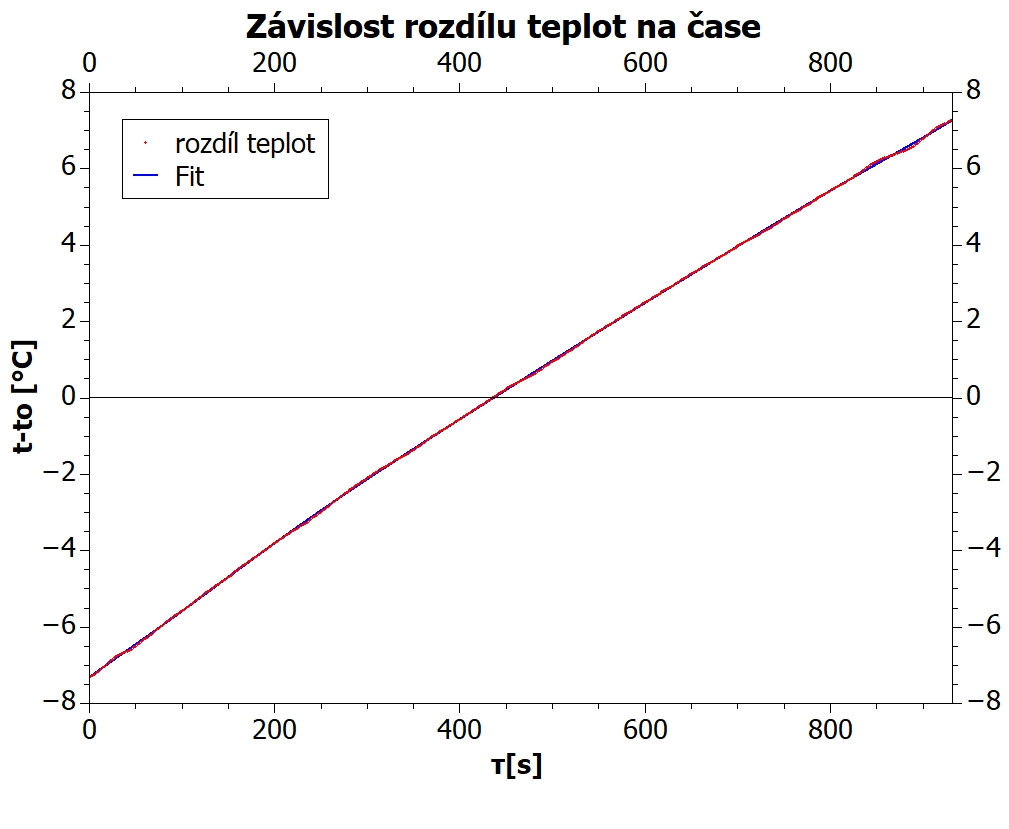
\includegraphics[width=0.6\linewidth, ]{ts} 
	\end{center}
	
	Proložíme-li graf hodnot polynomem, můžeme tuto spojitou funkci integrovat a následně získat tepelné ztráty podělené chladící konstantou (jelikož její hodnotu neznáme):
	\begin{equation}
		\frac{Q_s}{\beta} = \int a_0 + a_1 \tau + a_2 \tau ^2 + a_3 \tau ^3 d \tau 
	\end{equation}
	Při zafixování spodní meze a proměnné horní mezi hledáme hodnotu $\tau _2$, při které bude integrál velice blízko nule. Při $\tau = 890\, $s získáváme hodnotu $\frac{Q_s}{\beta} = 0 \pm 50$. (Od výše zmíněného předpokladu (5) se tento výsledek liší pouze o cca. deset sekund - předpoklad by byl splněn po $931.7\,$s experimentu.)
	
	
	
	  
  \subsection{Tepelné ztráty pomocí kalorimetrické rovnice}

	$m = 0.4006$ kg vody je ohřáto z počáteční teploty $t_p = 13.83\,$°C na teplotu $t_k = 27.74\, $°C výkonem $P = 30.2\,$W za dobu $\tau = 888.8\,$ s. Získaná kapacita kalorimetru je $K = 234\,\rm J.K^{-1}.kg^{-1}$
	Po dosazení do vzorce uvažujícího tepelné ztráty (při použití tabulkové hodnoty tepelné kapacity vody) získáme:
	\begin{equation}
		Q_s = P \tau - (mc + K)(t_k - t_p) = 260 \pm 150 \,\rm J
	\end{equation}
	Což je v porovnání s cca $30 \,$kJ dodaného tepla \textbf{velmi} uspokojivá hodnota
	

	\section{Tepelná kapacita vody}
	Se získanými veličinami můžeme spočítat dle rovnice (2) tepelnou kapacitu vody:
	\begin{equation}
		c = \frac{\frac{P \tau - Q_s}{t_k - t_p} - K}m = 4231 \pm 28 \,\rm J. ^\circ C ^{-1}.kg^{-1}
	\end{equation}
	
	
	\section{Závěr}
	Z experimentu vyplývá, že při správném uspořádání pokusu elektrického kalorimetru s cílem minimalizace tepelných ztrát lze dosáhnout výsledku, který bude mít přijatelnou hodnotu i bez zohlednění tepelných ztrát.
	
	% Nakonec nezapomeňte projet text programem vlna nebo vlnka, např.
	% 	vlna -m -l -n mojeuloha.tex
	% nebo zkontrolovat a opravit jednopísmenné předložky na koncích řádků ručně.
	
	
\end{document}
